\subsection{Prototypfilter}
\label{sec:Protototypfilter}

Bei jeder Filterdimensionierung wird von einem Prototypfilter ausgegangen, welches üblicherweise in der Form eines normierter Tiefpassfilters vorliegt. Abb.\ref{fig:Prototyp_Filter} zeigt die Topologie eines möglichen Tiefpassfilters (a) mit zugehöriger dualer Topologie (b).

\begin{figure}[h!]
\centering
 	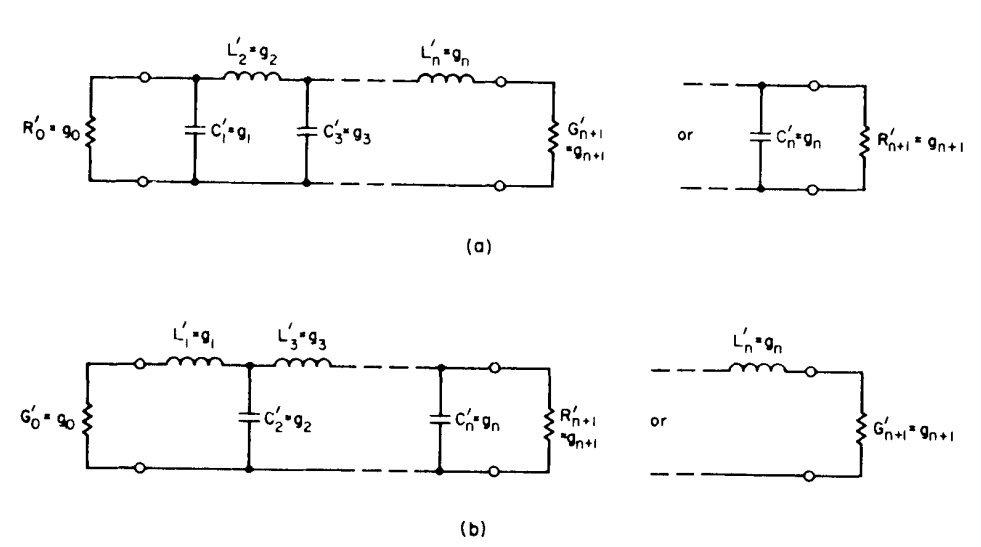
\includegraphics[width=\imagewidth]{images/Prototyp_Filter.png}
 	\caption{Topologie eines Prototyfilters (Tiefpass), Auszug aus dem Buch Microwave Filters, Impedancematching Networks and Coupling Structures \cite[p.~95]{ref:matthaei} }
 	\label{fig:Prototyp_Filter}
\end{figure}



Die Werte $g_0$ bis $g_{n+1}$ sind die Elementwerte des Protottypfilters. Diese Elementwerte können aus Tabellen entnommen werden und sind so normiert, dass das beschriebene  Prototypfilter die Grenzfrequenz $\omega_{C} = 1$, sowie die Lastimpedanz (oder Lastadmittanz) von $g_{n+1}=\SI{1}{\ohm} (\SI{1}{\siemens})$ aufweist. Dadurch kann der Prototyp sehr einfach in ein konkretes LC-Filter mit der gewünschten Lastimpedanz und Grenzfrequenz umgerechnet werden. 

Die Umrechnung in ein konkretes LC-Filter mit einer Lastimpedanz $Z_0$ und einer Grenzfrequenz $\omega_{C} = 1$ wird auch Entnormierung genannt und kann mit folgenden Formeln bewerkstelligt werden: 

\begin{equation}\label{eq:R}	
R_i = R'_i \cdot Z_0
\end{equation}

\begin{equation}\label{eq:L}	
L_i = \frac{L'_i \cdot Z_0}{\omega_{C}}
\end{equation}

\begin{equation}\label{eq:C}	
C_i = \frac{C'_i}{Z_0 \cdot \omega_{C}}
\end{equation}

Dabei beschreiben  $R'_i$, $C'_i$ und $L'_i$ die normierten Elementwerte  $g_0$ bis $g_{n+1}$ und $R_i$, $C_i$, und $L_i$ die konkreten Werte nach der Entnormierung.
